\documentclass[11pt,border=5pt]{standalone}
\usepackage{fontspec}
\setmainfont{cmunrm.otf}[BoldFont=cmunbx.otf,ItalicFont=cmunti.otf,BoldItalicFont=cmunbi.otf]
\usepackage{amsmath}
\usepackage{unicode-math}
\setmathfont{NewCMMath-Regular.otf}
\usepackage{tikz}
\usetikzlibrary{arrows.meta,patterns,angles,quotes}
\begin{document}
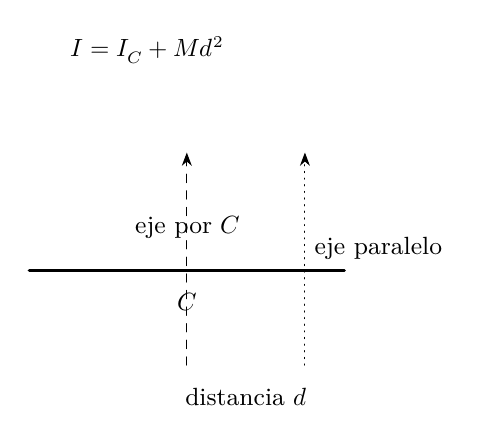
\begin{tikzpicture}[>=Stealth,font=\small,line cap=round,line join=round]
\draw[very thick] (-2,0) -- (2,0);
\draw[->,thin,dashed] (0,-1.2) -- (0,1.5) node[pos=0.55,above] {eje por $C$};
\draw[->,thin,dotted] (1.5,-1.2) -- (1.5,1.5) node[pos=0.55,right] {eje paralelo};
\node at (0,-0.4) {$C$};
\node at (0.75,-1.6) {distancia $d$};
\node at (-0.5,2.8) {$I=I_C+Md^2$};

\end{tikzpicture}
\end{document}
